%----------------------------------------------------------------
%
%  File    :  survey.tex
%
%  Author  :  Keith Andrews, IICM, TU Graz, Austria
%
%  Created :  24 Mar 2010
%
%  Changed :  22 Nov 2016
%
%----------------------------------------------------------------


\documentclass[11pt,onecolumn,twoside]{report}

\usepackage[          % set page and margin sizes
  a4paper,
  twoside,
  top=5mm,
  bottom=10mm,
  inner=15mm,
  outer=15mm,
  bindingoffset=10mm,
  head=10mm,
  foot=10mm,
  headsep=15mm,
  footskip=15mm,
  includeheadfoot,
]{geometry}
% A4 is 210 x 297 mm


\usepackage{txfonts}            % new times fonts
\usepackage{relsize}            % relative font sizes \smaller \larger

\usepackage[T1]{fontenc}        % 8-bit output chars (must be before inputenx)
\usepackage[utf8]{inputenx}     % input char encoding

\usepackage{float}              % H for float placement
\usepackage{setspace}           % line spacing

\usepackage{textcomp}           % symbols such as \texttimes and \texteuro
\usepackage{latexsym}

\usepackage{siunitx}            % prettier number formatting
\sisetup{%
  group-separator={,},
}
\usepackage[super]{nth}         % 1st, 2nd, 3rd, etc.

\usepackage{xspace}
\usepackage{etoolbox}           % for \newrobustcmd
\usepackage{makecmds}           % for \makecommand


\usepackage[english,austrian,british]{babel}

\usepackage[bf,sf]{titlesec}



\setlength{\textfloatsep}{10mm plus 2mm minus 1mm}
\setlength{\floatsep}{10mm plus 2mm minus 1mm}
\setlength{\intextsep}{10mm plus 2mm minus 1mm}

\setlength{\dbltextfloatsep}{10mm plus 2mm minus 1mm}
\setlength{\dblfloatsep}{10mm plus 2mm minus 1mm}

\setlength{\abovecaptionskip}{4mm plus 2mm minus 1mm}
\setlength{\belowcaptionskip}{0mm}




% use caption and subfig (caption2 and subfigure are now obsolete)

\usepackage[
  position=bottom,
  margin=1cm,
  font=small,
  labelfont={bf,sf},
  format=hang,
  indention=0mm,
]{caption,subfig}

\captionsetup[subfigure]{
  margin=0pt,
  parskip=0pt,
  hangindent=0pt,
  indention=0pt,
  singlelinecheck=true
}


\usepackage{tabu}

% fancyhdr to make nice headers and footers
% and deal with long chapter names

\usepackage{fancyhdr}         % headers and footers
\pagestyle{fancy}             % must call to set defaults before redefining

\renewcommand{\chaptermark}[1]{%
  \markboth{\thechapter.\ #1}{}
}
\renewcommand{\sectionmark}[1]{%
  \markright{\thesection.\ #1}
}
\renewcommand{\headrulewidth}{0mm}
\renewcommand{\footrulewidth}{0mm}
\newcommand{\headlook}{\sffamily}
\fancyhf{}
\fancyhead[LE,RO]{\thepage}
\fancyhead[LO]{%
\parbox[t]{0.8\textwidth}{\headlook\nouppercase{\rightmark}}
}
\fancyhead[RE]{%
\parbox[t]{0.8\textwidth}{\raggedleft\headlook\nouppercase{\leftmark}}
}


%\fancypagestyle{plain}{%   redefine plain style, but doesn't work
%  \fancyhf{}    % clear all header and footer fields
%  \fancyfoot[C]{\headlook \thepage} % except the center
%  \renewcommand{\headrulewidth}{0pt}
%  \renewcommand{\footrulewidth}{0pt}
%}



\usepackage{xcolor}
\definecolor{darkgreen}{rgb}{0.0,0.2,0.0}
\definecolor{darkblue}{rgb}{0.0,0.0,0.2}
\definecolor{darkred}{rgb}{0.2,0.0,0.0}
\definecolor{verylightgrey}{gray}{0.95}
\definecolor{lightgrey}{gray}{0.9}
\definecolor{black}{gray}{0.0}


\usepackage{tabularx}


\usepackage{listings}                 % for listings of source code
\usepackage{calc}                     % for calculation below

\makeatletter
\newlength{\numwidth}%
\setlength{\numwidth}{\widthof{\normalfont{\lst@numberstyle{99}}}}% Up to 2-digit (99) line numbers
\def\lst@PlaceNumber{%
  \makebox[\numwidth+1em][l]{%
    \makebox[\numwidth][r]{\normalfont\lst@numberstyle{\thelstnumber}}%
  }%
}
\makeatother

\lstset{                              % set parameters for listings
  floatplacement=tp,                  % default float placement
  numberbychapter,
  inputencoding=utf8,
  language=,                          % empty = plain text
  basicstyle=\small\ttfamily,
  tabsize=2,
  xleftmargin=1cm,
  xrightmargin=1cm,
  frame=none,
  framexleftmargin=0mm,
  rulesepcolor=\color{verylightgrey},
  numbers=none,
  numberstyle=\scriptsize,
  numbersep=2ex,
  breaklines,
  showtabs=false,
  showspaces=false,
  showstringspaces=false,
  keywordstyle=\bfseries,
  identifierstyle=,
  stringstyle=,
  captionpos=b,
  abovecaptionskip=\abovecaptionskip,
  belowcaptionskip=\belowcaptionskip,
  aboveskip=\floatsep,
  belowskip=\floatsep,
  extendedchars=true,
  literate=%
    {©}{{\textcopyright}}1
    {€}{{\texteuro}}1
    {Ö}{{\"O}}1
    {Ä}{{\"A}}1
    {Ü}{{\"U}}1
    {ß}{{\ss}}1
    {ö}{{\"o}}1
    {ä}{{\"a}}1
    {ü}{{\"u}}1,       % map some utf8 chars to replacements
}


\lstdefinelanguage{biblatex}   % based on biblatex v 2.7a from 2013-07-14
{
  keywords={%
    @article,@book,@mvbook,@inbook,@bookinbook,@suppbook,%
    @booklet,@collection,@mvcollection,@incollection,@suppcollection,%
    @manual,@misc,@online,@patent,@periodical,@suppperiodical,%
    @proceedings,@mvproceedings,@inproceedings,@reference,@mvreference,%
    @inreference,@report,@set,@thesis,@unpublished,@xdata,%
    @conference,@electronic,@mastersthesis,@phdthesis,@techreport,@www,%
    @artwork,@audio,@bibnote,@commentary,@image,@jurisdiction,@legislation,%
    @legal,@letter,@movie,@music,@performance,@review,@software,%
    @standard,@video%
  },
  comment=[l][\itshape]{@comment},
  sensitive=false,
}


\usepackage[short]{datetime}   % load datetime *after* babel, requires fmtcount
% \newdateformat{britdate}{%
% \ordinaldate{\THEDAY} \,\monthname[\THEMONTH] \THEYEAR
% }
\newdateformat{keithdate}{%
\twodigit{\THEDAY}~\shortmonthname[\THEMONTH]~\THEYEAR
}


\usepackage[hyphens,obeyspaces]{url}
\def\UrlFont{\smaller\ttfamily}



\usepackage[
  autostyle,
  english=british,
  threshold=0,
  thresholdtype=lines,
]{csquotes}
\renewcommand{\mkcitation}[1]{\space#1}

\newenvironment*{smallquote}          % smaller text within a block quote
  {\quote\smaller}
  {\endquote}
\SetBlockEnvironment{smallquote}

% put quotation marks around block quotes
% \renewenvironment{quoteblock}{\openautoquote}{\closeautoquote}

% I prefer double quotes as outer
\DeclareQuoteStyle[keithbritish]{british}%  [variant]{style}
  {\textquotedblleft}%                      opening outer mark
  {\textquotedblright}%                     closing outer mark
  [0.05em]%
  {\textquoteleft}%                         opening inner mark
  {\textquoteright}%                        closing inner mark

\setquotestyle[keithbritish]{british}



\usepackage[
  backend=biber,
  bibstyle=authoryear-ka,
  citestyle=authoryear-ka,
  sorting=nyt,
  useprefix,                   % van and von are part of second name
  mergedate=false,             % only for authoryear style
  dashed=false,                % only for authoryear style
  abbreviate=false,
  maxcitenames=2,              % if more than two authors, then use et al
  mincitenames=1,              % if exceeds 2 authors, then use 2
  maxbibnames=99,              % print all authors in biblio
  uniquename=init,
  hyperref=true,
  backref=true,
  backrefstyle=two,
  natbib=true,
  sortlocale=en,
]{biblatex}



% set for csquotes, but \autocite only available
% after biblatex is loaded
\SetCiteCommand{\autocite}    % or maybe \parencite

% more space between entries in bib
\setlength\bibitemsep{1.5\itemsep}


% remove URL: from in front of URLs
\DeclareFieldFormat{url}{\url{#1}}
\DeclareFieldFormat{doi}{\doi{#1}}
\DeclareFieldFormat{isbn}{\isbn{#1}}
\DeclareFieldFormat{issn}{\issn{#1}}

% suppress urldate field
\DeclareSourcemap{
  \maps[datatype=bibtex]{
    \map{
      \step[fieldset=urldate, null]
    }
  }
}

% for article titles
\DeclareFieldFormat{title:article}{\emph{#1}\midsentence}

\DefineBibliographyStrings{british}{%
  january          = {Jan},
  february         = {Feb},
  march            = {Mar},
  april            = {Apr},
  may              = {May},
  june             = {Jun},
  july             = {Jul},
  august           = {Aug},
  september        = {Sep},
  october          = {Oct},
  november         = {Nov},
  december         = {Dec},
}



% \bibliography{kandrews,latex,writing,inm-plag}

\addbibresource{writing.bib}
\addbibresource{latex.bib}
\addbibresource{kandrews.bib}
\addbibresource{ivis.bib}




\usepackage{ifpdf}

\ifpdf
  % pdflatex
  \usepackage[pdftex]{graphicx}
  \DeclareGraphicsExtensions{.pdf,.jpg,.png}
  \pdfcompresslevel=9
  \pdfpageheight=297mm
  \pdfpagewidth=210mm
  \usepackage[         % hyperref should be last package loaded
    unicode,
    pdftex,
    pdftitle={Writing a Survey Paper},
    pdfsubject={},
    pdfauthor={Keith Andrews},
    pdfkeywords={Master's Thesis, skeleton, guidelines, template},
    bookmarks,
    bookmarksnumbered,
    linktocpage,
    colorlinks,
    linkcolor=darkred,
    anchorcolor=red,
    citecolor=darkgreen,
    urlcolor=darkblue,
    pdfview={FitH},
    pdfstartview={Fit},
    pdfpagemode=UseOutlines,       % open bookmarks in Acrobat
    plainpages=false,              % avoids duplicate page number problem
    pdfpagelabels,                 % avoids duplicate page number problem
    breaklinks=true,               % allow links exceeding a single line
  ]{hyperref}

\else
  % latex
  % should never have to run latex, since l2h now understands pdflatex .aux
  \usepackage[dvips]{graphicx}
  \usepackage[dvips]{hyperref}
  \DeclareGraphicsExtensions{.eps}
\fi





% \liintro list item intro is a style used when list items have an
% introduction phrase (say in italics) followed by a colon.
\newcommand{\liintro}[1]{\emph{#1}}


\newcommand{\imgcredit}[1]
{\smaller{}[#1]}



\newcommand{\copyrightACM}
{%
Copyright \copyright\ by the Association for Computing Machinery, Inc.%
}




\newcommand{\daymonthyear}[3]
{%
\twodigit{#1}\hspace{0.7ex}\nolinebreak[2]\shortmonthname[#2]\hspace{0.7ex}\nolinebreak[2]#3%
}


\newcommand{\monthyear}[2]
{%
\shortmonthname[#1]\hspace{0.7ex}\nolinebreak[2]#2%
}


\newcommand{\yearmonthday}[3]
{%
\twodigit{#3}\hspace{0.7ex}\nolinebreak[2]\shortmonthname[#2]\hspace{0.7ex}\nolinebreak[2]#1%
}


\newcommand{\yearmonth}[2]
{%
\shortmonthname[#2]\hspace{0.7ex}\nolinebreak[2]#1%
}



% link to Amazon or
% http://worldcatlibraries.org/wcpa/isbn/[ISBN number]

\newrobustcmd{\isbn}[1]
{%
{%
\ifpdf
{\smaller ISBN}
\href{http://www.amazon.com/exec/obidos/ASIN/#1/keithandrewshcic}{#1}%
\else
{\smaller ISBN}
#1%
\fi
}%
}



% ISSN
% http://www.bl.uk/services/bibliographic/issn.html
% 8 digits, should be printed xxxx-xxxx
% e.g. 0020-0190 is Information Processing Letters, Elsevier
%
% Lookup services:
% http://kmittlib.lib.kmutt.ac.th:81/search/i?SEARCH=0020-0190
% http://worldcatlibraries.org/wcpa/issn/0020-0190

\newrobustcmd{\issn}[1]
{%
{%
\ifpdf
{\smaller ISSN}
\href{http://worldcatlibraries.org/wcpa/issn/#1}{#1}%
\else
{\smaller ISSN}
#1%
\fi
}%
}



% DOIs  http://www.doi.org/  e.g.
% doi:10.1038/nature723
% http://dx.doi.org/10.1038/nature723

\newrobustcmd{\doi}[1]
{%
{%
\def\UrlFont{\rmfamily}
\ifpdf                                   % pdflatex
\href{http://dx.doi.org/#1}{doi:\protect\nolinkurl{#1}}%
\else                                    % latex
doi:\protect\nolinkurl{#1}%
\fi
}%
}





\newrobustcmd{\website}[1]
{%
\ifpdf                                  % pdflatex
\href{http://#1/}{\nolinkurl{#1}}%
\else                                   % latex
\nolinkurl{#1}%
\fi
}




\newcommand{\news}[1]
{%
\ifpdf
\href{news:#1}{\nolinkurl{#1}}
\else
\nolinkurl{#1}%
\fi
}








% based on url package
% define styles for class, file, and variable names
% which break nicely at line breaks

% make the macros robust so they work inside captions, etc

\newcommand{\ttname}{\begingroup \smaller\urlstyle{tt}\Url}
\newcommand{\rmname}{\begingroup \smaller\urlstyle{rm}\Url}
\newcommand{\sfname}{\begingroup \smaller\urlstyle{sf}\Url}


% cname is for class names
\newrobustcmd{\cname}[1]{\sfname{#1}}

% fname is for file names and directory names
\newrobustcmd{\fname}[1]{\ttname{#1}}

% vname is for variable names, domain names, email addresses
\newrobustcmd{\vname}[1]{\ttname{#1}}



% Euro symbol
\newcommand{\euro}{\texteuro\,}

% times symbol
\newcommand{\timessym}{\texttimes\,}

% approx symbol
\newcommand{\approxsym}{\ensuremath\approx\,}

% plusminus symbol
\newcommand{\plusminussym}{\textpm\,}

% not equal symbol
\newcommand{\neqsym}{\ensuremath{\neq\,}}

% rightarrow symbol
\newcommand{\rightarrowsym}{\ensuremath\rightarrow\,\,}




\newcommand{\TODO}[1]
{
{\textcolor{red}{[TODO: #1]}}
}



\newcommand{\fullh}{18cm}         % height of figures for 1 per page
\newcommand{\halfh}{9.5cm}        % height of figures for 2 per page
\newcommand{\thirdh}{6cm}         % height of figures for 3 per page


\tolerance=400 
  % makes some lines with lots of white space, but      
  % tends to prevent words from sticking out in the margin






\begin{document}

\keithdate

\normalsize
\pagestyle{empty}         % for preliminary pages (no numbers shown)
\pagenumbering{Roman}     % for pdf labels




\begin{titlepage}

\begin{center}
{\Large \sffamily \bfseries Matrix Representation of Graphs}

\vspace{1cm}

{\large\sffamily Group 3\\ \vspace*{1cm}}
{\small\sffamily 
Eva Rott\\
Michael Glatzhofer\\
Dominik Mocher\\
Julian Wolf
}

% {\large\sffamily Group 4}
% \vspace{5mm}
% {\large\sffamily Keith Andrews, Tom Strong, Bill Weak, and Seb Green}

\vspace{1cm}

Institute for Information Systems and Computer Media (IICM), \\
Graz University of Technology \\
A-8010 Graz, Austria \\[1cm]


% {\large
% 706.057 Information Visualisation SS 2016 \\
% Graz University of Technology \\[1cm]
% }

\vspace{1cm}

{\large 15 Mai 2017}

\end{center}



\vspace{2cm}

\begin{quote}
\begin{center}
{\large\sffamily\bfseries Abstract}
\end{center}

By representing graphs in a matrix adjancy matrix it is possible to observe special patterns and reveal dependencies which might not be seen in the graph per se. By combining the benefits of both the matraix representation and the graph it self, a very powerfull approach of graph analysing may be achieved. 

In this survey we present some powerfull techniques applyable to adjancy matrices to analyze graphs. furthermore, we present some tools utilizing these techniques.

\end{quote}

\vfill

\begin{center}
{\small\sffamily \copyright ~ Copyright 2016 by the author(s),
except as otherwise noted.}

\vspace{2mm}
{\footnotesize\sffamily This work is placed under a
Creative Commons Attribution 4.0 International
(\href{https://creativecommons.org/licenses/by/4.0/}{CC BY 4.0}) licence.}
\end{center}

\end{titlepage}




\cleardoublepage
\pagestyle{plain}
\pagenumbering{roman}



{
\setlength{\parskip}{3pt plus 3pt minus 3pt}     % compact tables of contents
\tableofcontents
\addcontentsline{toc}{chapter}{Contents}

\cleardoublepage
\listoffigures
\addcontentsline{toc}{chapter}{List of Figures}

\cleardoublepage
\listoftables
\addcontentsline{toc}{chapter}{List of Tables}

\cleardoublepage
\renewcommand{\lstlistlistingname}{List of Listings}
\lstlistoflistings
\addcontentsline{toc}{chapter}{List of Listings}
}


\cleardoublepage
\pagestyle{headings}        % for main pages
\pagenumbering{arabic}


\cleardoublepage
%----------------------------------------------------------------
%
%  File    :  survey-intro.tex
%
%  Author  :  Keith Andrews, IICM, TU Graz, Austria
% 
%  Created :  27 May 1993
% 
%  Changed :  16 Nov 2010
% 
%----------------------------------------------------------------


\chapter{Basics}\label{chap:Basics}


This chapter explains the different types of graphs and their corresponding matrices, which techniques are basically used on matrices and how to interpret the resulting patterns

\section{Definitions}
Every node in the graph has its distinctive unique id, which never changes. In this paper, the terms ``nodes" and ``edges" are used. 

\textbf{TODO: some more stuff here}




\section{Types of Graphs}

We distinguish between two types of edges (directed and undirected) and two types of cost calculations (weighted and unweighted) between the nodes, which leads to 4 different graphs

\subsection{directed/undirected}

As can be seen in figure~\ref{fig:dir_graph} undirected edges may be traversed in any direction, whereas directed edges may just be traversed in one direction. 

\textbf{TODO: some more stuff here}

\subsection{weighted/unweighted}

A graph without weights has uniform costs on all edges, which leads to equal costs by traversing the edges in any order. When adding weights or costs to the edges, this fact changes. The order or selection of traversing the edges does matter as it creates different costs.


\textbf{TODO: some more stuff here}

\section{Use cases}
Some use cases of the different graph types are (to name just a few examples):
\begin{itemize}
\item Navigation system (weighted directed)
	\begin{itemize}
		\item Nodes: Cities/POIs
		\item Edges: Routes directed (one way streets)
		\begin{itemize}
			\item weights
			\begin{itemize}
				\item length of street (find shortest way)
				\item time to traverse the street (find fastest way)
			\end{itemize}		
		\end{itemize}
	\end{itemize}		
\item Subway map (undirected unweighted)
\begin{itemize}
	\item Nodes: stations
	\item edges: connection between stations
\end{itemize}
\item Relations of tweets (directed unweighted)
\begin{itemize}
	\item nodes: single tweet entry
	\item edges: references to other tweets
\end{itemize}
\end{itemize}




\section{Matrix representation of graphs}

When representing graphs in a matrix, an adjacency matrix is used. Adjacency matrices are structured with every row and every column represents one node. This leads to a N x N square matrix, where N is the number of nodes. 

These matrices show some patterns according to their corresponding graph but most times these patterns are not immediately visible. There are some techniques to reveal these patterns, all of them involving the reordering of the matrix.


\subsection{Reordering}

The main goal of reordering the matrix is to cluster the edges and thus reveal certain patterns. An example of this behaviour can be seen in figure~\ref{fig:reorder}. 

\begin{figure}[h]
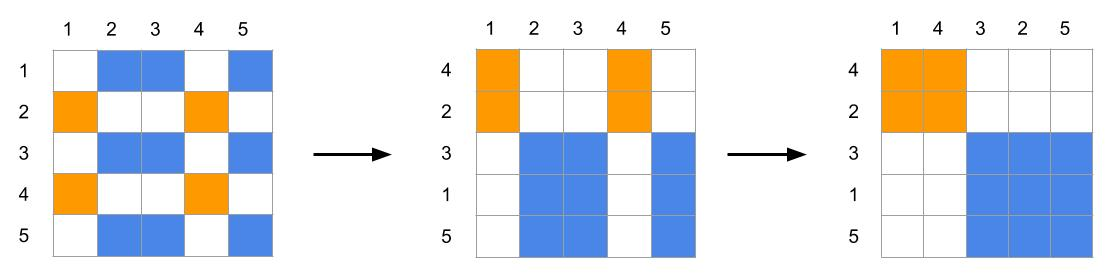
\includegraphics[width=\textwidth]{images/reorder}
\caption{Reordering a matrix\label{fig:reorder}}
\end{figure}


When reordering the matrix, the indices of the single rows and columns stay with the rows, otherwise the graph would change by this workstep. In this example, at first the rows 1 and 4 get swapped and as a second step columns 2 and 4. In this way the full connection pattern of the two subgraphs may be observed. 

\subsection{Patterns}
There are 4 main patterns which may be revealed by reordering the matrix. These patterns may be combined in such a way, that for example a subgraph creates a circle, but one node if it is connected to every other node. This results in a combination of the star and the circle pattern. 
The four different patterns can be seen in the corresponding figures~\ref{fig:patterns}.
\begin{table}
  \centering
\begin{tabu}{cc}
	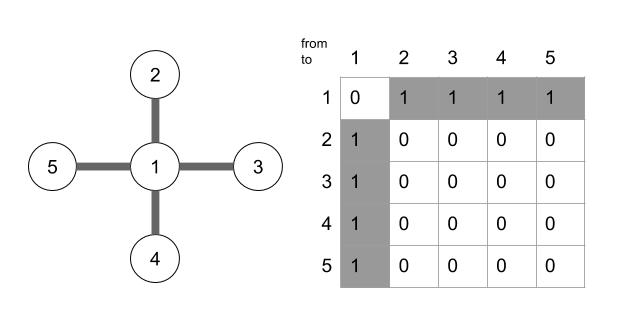
\includegraphics[width=0.49\textwidth]{images/pattern_star}  &
	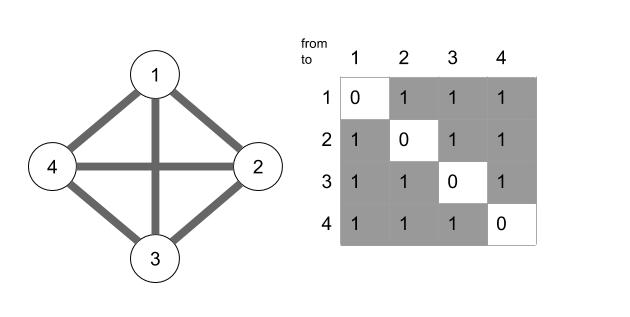
\includegraphics[width=0.49\textwidth]{images/pattern_full} \\
	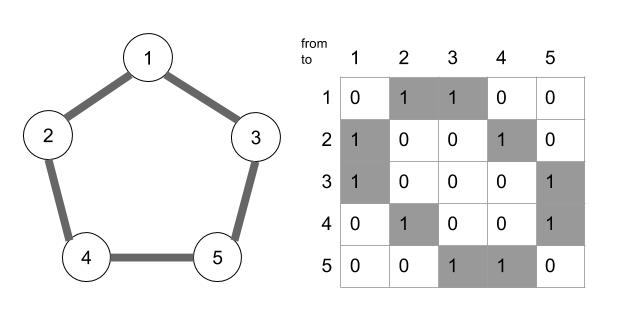
\includegraphics[width=0.49\textwidth]{images/pattern_circle} &
	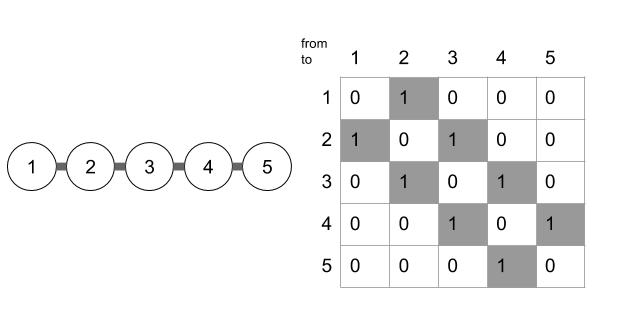
\includegraphics[width=0.49\textwidth]{images/pattern_line} 
\end{tabu}
\captionof{figure}{4 differnet patterns: star, full, circle and line\label{fig:patterns}}
\end{table}



\cleardoublepage
%----------------------------------------------------------------
%
%  File    :  survey-browsers.tex
%
%  Author  :  Keith Andrews, IICM, TU Graz, Austria
% 
%  Created :  27 May 1993
% 
%  Changed :  16 Nov 2010
% 
%----------------------------------------------------------------


\chapter{Hierarchy Browsers}

\label{chap:Browsers}


If the survey were on the topic of hierarchy browsers, for example,
this is how I might divide up the field.



\section{Node-Link Hierarchy Browsers}

\subsection{Layered}

\subsection{Radial}





\section{Space-Filling Hierarchy Browsers}

\subsection{Layered}

\subsection{Radial}

\subsection{Inclusive}

\subsection{Overlapping}






\section{Evaluating Hierarchy Browsers}

\subsection{Formative Studies}

\subsection{Comparative Studies}





\cleardoublepage
%----------------------------------------------------------------
%
%  File    :  survey-academic.tex
%
%  Author  :  Keith Andrews, IICM, TU Graz, Austria
% 
%  Created :  27 May 93
% 
%  Changed :  22 Oct 2012
% 
%----------------------------------------------------------------


\chapter{Academic Writing}

\label{chap:Academic}




Writing in an academic context is different to other types of
writing. Care must be taken to follow the conventions of academic
writing.



\section{Academic Criteria}

An academic survey must demonstrate the following components:
\begin{itemize}
\item Motivation. What problem you are addressing and why.

\item Survey. A thorough review of related work in the field.

\item An extensive bibliography. To demonstrate knowledge of the major
  works in the field, even if they have not all been read in their
  entirety.
\end{itemize}






\section{Academic Integrity}

It is very easy to find helpful material on the web. Resist the
temptation to copy such material verbatim, even with minor changes in
phrasing and word order. It is just as easy for a supervisor or
advisor (or anyone else for that matter) to check the originality of a
piece of text by copying a passage into Google or services such as
\citep{PlagiarismOrg}.

Work submitted for academic assessment must be original and created by
the stated author(s). Care must be taken to avoid both
\emph{plagiarism} and \emph{breach of copyright}:
\begin{itemize}
\item \liintro{Plagiarism}: Using the work of others \emph{without
  acknowledgement}.

\item \liintro{Breach of copyright}: Using the work of others
  \emph{without permission}.
\end{itemize}






\subsection{Plagiarism}

Plagiarism is a violation of intellectual honesty. This means copying
other people's work or ideas without due acknowledgement, thus giving
the reader the impression that these are original (your own) work and
ideas. The Concise Oxford Dictionary, 8th Edition, defines plagiarism
as:
\begin{quotation}
\noindent
``\textbf{plagiarise}
\textbf{1} take and use (the thoughts, writings, inventions, etc.\ of
another person) as one's own. \textbf{2} pass off the thoughts etc.\
of (another person) as one's own.''
\end{quotation}
Plagiarism is the most serious violation of academic integrity and can
have dire consequences, including suspension and expulsion
\citep{Reisman2005}.



\subsection{Breach of Copyright}

Copyright law\footnote{Disclaimer: I am not a lawyer. The comments
  here reflect the situation to the best of my knowledge at the time
  of writing, but do not constitute legal advice. Laws sometimes
  change and I make no guarantees.} varies in detail from country to
country, but certain aspects are internationally widely accepted. In
general, the creator of a work, say a piece of writing, a diagram, a
photograph, or a screenshot, automatically has copyright of that
work. Copyright usually expires 70 years after the creator's
death. The copyright holder can grant the right for others to use or
publish their work on an exclusive or non-exclusive basis.

The copyright laws of most countries have provisions for \emph{fair
  use}, which generally means it is allowable to quote small parts of
a work. Austrian copyright law \citep[§ 42f]{UrhG} allows for
reasonable quotes from published works or works made publicly
available with permission of the copyright holder. Austrian copyright
law \citep[§ 42g]{UrhG} also makes certain exemptions for materials
used for teaching in universities and schools. Note that significant
changes to Austrian copyright law \citep{UrhG-Novelle-2015} came into
effect on \yearmonthday{2015}{10}{1}.





\section{Acceptable Use}

Academic work almost always builds upon the work of others, and it is
appropriate, indeed essential, that related and previous work by
others be discussed in an academic thesis. However, this must be done
according to the rules of acceptable use. There are two forms of
acceptable use:
\begin{itemize}
\item \liintro{Paraphrasing (Indirect Quotation)}: Summarising the ideas
  of someone else using original words and with attribution.
\item \liintro{Quoting (Direct Quotation)}: Including an exact
  verbatim copy inside quotation marks and with attribution.
\end{itemize}
Attribution means that the original source is cited.
For further information on acceptable and non-acceptable academic
practice see \citep{FremdeFedern,Wikipedia-Zitat}.




\subsection{Paraphrasing (Indirect Quotation)}

Paraphrasing means closely summarising and restating the ideas of
another person, but in (your own) original words. When writing a
literature survey, the relevant parts of each paper or source are
generally \emph{paraphrasd}.

One good technique for paraphrasing is:
\begin{enumerate}
\item Read the original source.
\item Put it down away from view.
\item \emph{Without refering to the original}, summarise it in your own words.
\end{enumerate}
When paraphrasing someone else's ideas, the original source must
always be cited!

Since paraphrased text is not enclosed in quotation marks, it is not
always obvious how to indicate the extent of the text which
corresponds to a particular citation. If the paraphrased text only
covers a single paragraph, include the citation either within or at
the end of the first sentence of the paragraph, or at the end of the
paragraph. Otherwise, describe the extent of the citation in words at
the beginning, for example: This section is based on the work of
\citet{InfoSkyIVS}.




\subsection{Quoting Text (Direct Quotation)}

In some circumstances, it makes sense to directly \emph{quote} small
parts of text (typically a few sentences or paragraphs) from a
relevant source. When quoting directly, the \emph{exact} words,
spelling, and punctuation of the original are copied verbatim and
enclosed in quotation marks.

Most of an academic paper or thesis must be in words written by the
author(s) themselves. However, when an exact phrase or specific
wording from another source is important, then a direct quotation
should be used. In any case, the original source must be cited!




\subsection{Quoting Images}

It is common to want to include photographs, diagrams, or screenshots
taken from the internet or from another work, particularly when
surveying related work. Austrian copyright law \citep[§ 42f]{UrhG}
allows images from published works to be included in scientific works
for the purposes of discussion. However, it is not entirely clear what
constitutes a scientific work and what not. The safest policy is
always to ask permission from the owner.

For diagrams, an alternative strategy is to redraw and possibly adapt
the diagram in a drawing editor such as Adobe Illustrator
\citep{Adobe-Illustrator} or Inkscape \citep{Inkscape}. The original
source should be cited with wording like ``Redrawn from [\ldots]'' or
``Adapted from [\ldots]''.

For graphs and plots, it is often possible to reconstruct the graphic
from the original data using tools such as gnuplot \citep{gnuplot} or
R \citep{R-Project}. The original source should be cited with wording
similar to ``Created from the original data [\ldots] using[\ldots]''.

For screenshots, it is sometimes possible to obtain the original
software, install it, and make new screenshots. The source software
should be cited with wording similar to ``Screenshot created using
[\ldots]''.




\subsection{Always State Both Source and Permission}

Regardless of whether permission has been obtained from the copyright
owner or material is being used under the provisions of a specific
country's copyright law: whenever someone else's work is being used,
academic integrity dictates that the original source must be cited!
In addition, it is also good practice to state the terms (permission)
under which the material is being used.


For each piece of included material, make two things absolutly clear:
\begin{enumerate}
\item \liintro{Source}: Cite the original source of the material.
  Use a standard \LaTeXe citation.

\item \liintro{Permission}: Explain the legal basis for using the
  material. For example, give the \emph{exact} Creative Commons
  licence, state the \emph{exact} legal exemption, or state that
  permission has kindly been given by the named original author.
\end{enumerate}


These two things should be stated in two places:
\begin{itemize}
\item \liintro{Caption}: At the end of the caption of the figure
  or listing.

\item \liintro{Credits section}: In the Credits section at the
  front of the thesis.
\end{itemize}


All this means, of course, that if a thesis is based upon this
skeleton \citep{KeithThesis}, then the source and permission should be
stated at the appropriate place (in this case, in the Credits
section).







\section{References}



\subsection{Bib Files}

Typically, one or more \vname{.bib} files are prepared, containing
various original sources and references.
Listing~\ref{list:BibFile} shows four typical entries from a
\vname{.bib} file for use with biblatex and biber. The
\vname{inproceedings} entry describes a paper published in conference
proceedings, the \vname{article} entry describes a paper published in
a journal, and the \vname{booklet} entry is being used for internet
resources and web sites (\vname{booklet} has the advantage over
\vname{online} that it has a \vname{howpublished} field.).



\lstinputlisting[%
  float=tp,
  xleftmargin=0cm,              % no extra margins for floats
  xrightmargin=0cm,             % no extra margins for floats
  language=biblatex,
  basicstyle=\footnotesize\ttfamily,
  frame=shadowbox,
  numbers=left,
  label=list:BibFile,
  caption={[Four Typical Entries from a \vname{.bib} File]%
Four typical entries from a \vname{.bib} file for use
with biblatex and biber.
An \vname{inproceedings} entry describes a paper published
in conference proceedings, an \vname{article} entry describes
a paper published in a journal, and a \vname{booklet} entry
is used for internet resources and web sites.
The \vname{doi} field gives
the DOI (digital object identifier) of the paper.},
]
{listings/some.bib}


Of particular note is the \vname{doi} field, which gives the DOI
(digital object identifier) of a paper. DOIs are for academic papers
what ISBNs are for books; a unique handle with which one can easily
find the original. Most publishers are now assigning DOIs to new
conference and journal papers and are working back in time to assign
them to previously published papers. Always give the DOI of a paper
where one is available. If a DOI exists but points to a subscription
site, and the paper is also freely available on the web (say at the
home page of an author), then use the \vname{url} field to give the
free URL as well. Do not redundantly give the same URL in the
\vname{url} field which the DOI itself resolves to.





\subsection{Downloading Bib Entries}

\begin{lstlisting}[%
  float=tp,
  xleftmargin=0cm,              % no extra margins for floats
  xrightmargin=0cm,             % no extra margins for floats
  language=biblatex,
  basicstyle=\footnotesize\ttfamily,
  frame=shadowbox,
  numbers=left,
  label=list:BibACMIEEE,
  caption={[Massaging Bib Entries from ACM and IEEE]%
Bib entries copied from the ACM Digital Library or the
IEEE Computer Society Digital Library contain useful information,
but cannot be used ``as-is''. They must be edited to conform
to biblatex and to these thesis guidelines.
},
]
% From the IEEE Computer Society DL:

@article{10.1109/INFOVIS.2005.7,
author = {Martin Wattenberg},
title = {Baby Names, Visualization, and Social Data Analysis},
journal = {infovis},
volume = {0},
year = {2005},
issn = {1522-404x},
pages = {1},
doi = {http://doi.ieeecomputersociety.org/10.1109/INFOVIS.2005.7},
publisher = {IEEE Computer Society},
address = {Los Alamitos, CA, USA},
}


% From the ACM DL:

@inproceedings{1106568,
 author = {Martin Wattenberg},
 title = {Baby Names, Visualization, and Social Data Analysis},
 booktitle = {INFOVIS '05: Proceedings of the Proceedings of the 2005 IEEE Symposium on Information Visualization},
 year = {2005},
 isbn = {0-7803-9464-x},
 pages = {1},
 doi = {http://dx.doi.org/10.1109/INFOVIS.2005.7},
 publisher = {IEEE Computer Society},
 address = {Washington, DC, USA},
 }


% Clean, edited version for Keith:

@inproceedings{WattenbergNames,
  author       = "Martin Wattenberg",
  title        = "Baby Names, Visualization, and Social Data Analysis",
  booktitle    = "Proc.\ {IEEE} Symposium on Information Visualization
                  (InfoVis 2005)",
  location     = "Minneapolis, Minnesota, USA",
  organization = "{IEEE} Computer Society",
  isbn         = "078039464X",
  date         = "2005-10",
  pages        = "1--8",
  doi          = "10.1109/INFOVIS.2005.7",
  url          = "http://www.research.ibm.com/visual/papers/final-baby-margin-nocomments.pdf",
}
\end{lstlisting}



When \vname{.bib} entries are downloaded or copied from the ACM
Digital Library, the IEEE Digital Library, or other onlibne sources,
they should \emph{not} be used as is. They generally need to be
cleaned up first and made consistent with biblatex.
Listing~\ref{list:BibACMIEEE} shows typical BibTeX entries provided by
the ACM Digital Library and the IEEE Computer Society Digital Library.


To bring bib entries into line with biblatex and the examples shown in
Listing~\ref{list:BibFile}, the following should be addressed:
\begin{itemize}
\item The title of the paper should use capitalised main words.

\item Capitalisations in the title which need to be preserved (such as
  the R in VRwave) should be enclosed in curly brackets ({VRwave}).

\item The \vname{title} and \vname{booktitle} should use
  capitalised main words (not all lower case).

\item The \vname{edition} field is usually be a number in inverted
  commas, such as \verb|"2"|, instead of a word such as
  \verb|"Second"|.

\item The name of a conference should be rephrased, with the short
  form of the conference name in parentheses at the end (VRML'98).

\item Any \vname{year}, \vname{month}, and \vname{day}
  fields should be combined into a \vname{date} field.

\item For a conference paper, the first day of the conference
  should be used as the date of publication.

\item The location of a conference should be in the \vname{venue}
  field, not in the \vname{address} or \vname{location} field.
  The \vname{address} field is for the address of the publisher.


\item Any minus signs must be removed from the ISBN number.
  Otherwise, the macro used in this skeleton for handling ISBNs and
  linking to Amazon will break.

\item Any initial \vname{http://doi.acm.org/} or
  \vname{http://doi.ieeecomputersociety.org/} must be removed from
  the DOI. They are \emph{not} part of the DOI.

\item If a free, unofficial version of a paper with a DOI is available
  at the web site of one of the authors, give this in the \vname{url}
  field.

\item Manually shorten any URL as much as possible: try selectively
  removing parameters after a question mark and try removing
  \vname{www} from the domain. Do \emph{not} use a URL shortening
  service like \website{bit.ly}, since there is no guarantee the
  service will be around long term. It is acceptable to use a URL
  shortening service maintained by the original site themselves, such
  as \website{youtu.be} for YouTube URLs.

\end{itemize}






\subsection{What to Reference}

The set of references should be balanced:
\begin{itemize}
\item Do not have largely web sites as references. A few web sites as
  references is fine, most references being web sites is (usually) not
  so good.

\item Do not have too many Wikipedia references. A few Wikipedia
  references is OK; more than a few is not. Wikipedia is a good
  \emph{starting} point for (further) academic research, it is not a
  good ending point for academic research.

\item Have plenty of academic conference and journal papers (with a
  DOI). Sometimes, both an academic paper and a project web site will
  be avilable -- reference both as separate entries.

\item Include some books (with an ISBN) if at all possible. Books
  still count in academic circles.
 
\item If you know or suspect who will be reviewing or marking your
  thesis or paper, make sure to include some of their references. The
  first thing many reviewers do is check to see if they appear in the
  bibliography.

\item No ghost references. Every reference in the bibliography should
  be cited somewhere in the text.

\end{itemize}





\subsection{Citing}

When a citation is included within flowing text:
\begin{itemize}
\item Distinguish between \emph{textual} citations and
  \emph{parenthetical} citations. Textual citations are used to embed
  the authors' names in the current sentence. Parenthetical citations
  are used at the end of a sentence.
\begin{quote}
\verb|\citet{Jones1990}| \rightarrowsym Jones et al. [1990] \\
\verb|\citep{Jones1990}| \rightarrowsym [Jones et al., 1990]
\end{quote}


\item If one specific part in a very long paper or book is being
  cited, always state the page number or range in the citation:
\begin{quote}
\verb|As \citet[pages 22--23]{Jones1990} say| \rightarrowsym As Jones et al. [1990, pages 22–23] say\\
\end{quote}





\section{Guides to Scientific Writing}

\citet{CraftScientificWriting} is one of the classic guides to
scientific writing. Other good ones include \citet{BoothCraft}
and \citet{BoothCommunicating}.



\end{itemize}



\cleardoublepage
%----------------------------------------------------------------
%
%  File    :  survey-style.tex
%
%  Author  :  Keith Andrews, IICM, TU Graz, Austria
% 
%  Created :  27 May 93
% 
%  Changed :  19 Feb 2004
% 
%----------------------------------------------------------------


\chapter{Language and Writing Style}

\label{chap:Style}



The classic reference for English writing style and grammar is
\citet{StrunkWhite}. The original text is now available for free
online \citep{Strunk}, so there is no excuse at all for writing poor
English. Readers should consult it first, then continue reading this
chapter. Another good free guide is \citet{NASAGuide}.

\citet{Zobel-WritingCompSci} and \citet{BugsInWriting} are guides
specifically aimed at computer science students.
\citet{Phillips-HowGetPhD} gives practical advice for PhD
students. Sections~\ref{sec:Clear} and \ref{sec:Gender} are adapted
from the ACM CHI'94 conference language and writing style guidelines.




\section{Paragraphs}

Sentences should be grouped into paragraphs by topic. A new paragraph
introduces a (slight) variation in topic. Paragraphs should generally
consist of \emph{several} sentences. Short paragraphs of only one or
two sentences should be merged topically with neighbouring paragraphs.



\section{Some Basic Rules of English}

There are a few basic rules of English for academic writing, which are
broken regularly by my students, particularly if they are non-native
speakers of English. Here are some classic and often encountered
examples:

\begin{itemize}

\item \emph{Never} use I, we, or you.

Write in the passive voice (third person).

\begin{tabular}{lp{0.9\hsize}}
Bad:  & You can do this in two ways.   \\
Good: & There are two ways this can be done.  \\
\end{tabular}



\item \emph{Never} use he or she, his or her.

Write in the passive voice (third person).

\begin{tabular}{lp{0.9\hsize}}
Bad:  & The user speaks his thoughts out loud.   \\
Good: & The thoughts of the user are spoken out loud.  \\
\end{tabular}

See Section~\ref{sec:Gender} for many more examples.



\item Stick to a consistent dialect of English. Choose either
  British or American English and keep to it throughout the
  whole of your thesis.



\item Do \emph{not} use slang abbreviations such as ``it's'',
  ``doesn't'', or ``don't''.

Write the words out in full: ``it is'', ``does not'', and ``do not''.

\begin{tabular}{lp{0.9\hsize}}
Bad:  & It's very simple to\ldots       \\
Good: & It is very simple to\ldots       \\
\end{tabular}



\item Do \emph{not} use abbreviations such as ``e.g.'' or
  ``i.e.''. 

Write the words out in full: ``for example'' and ``that is''.

\begin{tabular}{lp{0.9\hsize}}
Bad:  & \ldots in a tree, e.g. the items\ldots        \\
Good: & \ldots in a tree, for example the items\ldots   \\
\end{tabular}



\item Do \emph{not} use slang such as ``a lot of''.

\begin{tabular}{lp{0.9\hsize}}
Bad:  & There are a lot of features\ldots       \\
Good: & There are many features\ldots       \\
\end{tabular}



\item Do \emph{not} use slang such as ``OK'' or ``big''.

\begin{tabular}{lp{0.9\hsize}}
Bad:  & \ldots are represented by big areas.    \\
Good: & \ldots are represented by large areas.  \\
\end{tabular}



\item Do \emph{not} use slang such as ``gets'' or ``got''.

Use ``becomes'' or ``obtains'', or use the passive voice (third
person).

\begin{tabular}{lp{0.9\hsize}}
Bad:  & The radius gets increased\ldots       \\
Good: & The radius is increased\ldots         \\
\end{tabular}

\begin{tabular}{lp{0.9\hsize}}
Bad:  & The user gets disoriented\ldots       \\
Good: & The user becomes disoriented\ldots    \\
\end{tabular}




\item \emph{Never} start a sentence with ``But''.

Use ``However,'' or ``Nevertheless,''. Or consider joining the
sentence to the previous sentence with a comma.

\begin{tabular}{lp{0.9\hsize}}
Bad:  & But there are numerous possibilities\ldots       \\
Good: & However, there are numerous possibilities\ldots  \\
\end{tabular}



\item \emph{Never} start a sentence with ``Because''.

Use ``Since'', ``Owing to'', or ``Due to''. Or turn the two
halves of the sentence around.




\item \emph{Never} start a sentence with ``Also''. Also should
be placed in the middle of the sentence.

\begin{tabular}{lp{0.9\hsize}}
Bad:  & Also the target users are considered. \\
Good: & The target users are also considered. \\
\end{tabular}



\item Do \emph{not} use ``that'' as a connecting word.

Use ``which''.

\begin{tabular}{lp{0.9\hsize}}
Bad:  & \ldots a good solution that can be computed easily.  \\
Good: & \ldots a good solution which can be computed easily.  \\
\end{tabular}




\item Do \emph{not} write single-sentence paragraphs. 

Avoid writing two-sentence paragraphs. A paragraph should contain at
least three, if not more, sentences.


\end{itemize}



% rules on the use of a comma in lists
% http://en.wikipedia.org/wiki/Serial_comma








\section{Avoid Austrianisms}
\label{sec:Austrianisms}


I see these mistakes time and time again. Please do not
let me read one of them in your work.



\begin{itemize}


\item ``actual'' \neqsym ``current'' 

If you mean ``aktuell'' in German, you probably mean
``current'' in English.

\begin{tabular}{lp{0.9\hsize}}
Bad:  & The actual selection is cancelled. \\
Good: & The current selection is cancelled. \\
\end{tabular}



\item ``allows to'' is not English.

\begin{tabular}{lp{0.9\hsize}}
Bad:  & The prototype allows to arrange components\ldots \\
Good: & The prototype supports the arrangement of components\ldots \\
\end{tabular}

% they allow to achieve



\item ``enables to'' is not English.

\begin{tabular}{lp{0.9\hsize}}
Bad:  & it enables to recognise meanings\ldots \\
Good: & it enables the recognition of meanings\ldots \\
\end{tabular}


\item ``according'' \neqsym ``corresponding'' 

\begin{tabular}{lp{0.9\hsize}}
Bad:  & For each browser, an according package is created. \\
Good: & For each browser, a corresponding package is created. \\
\end{tabular}



\item ``per default'' is not English.

Use ``by default''.

\begin{tabular}{lp{0.9\hsize}}
Bad:  & Per default, the cursor is red. \\
Good: & By default, the cursor is red. \\
\end{tabular}




\item ``As opposed to'' is not English.

Use ``In contrast to''.

\begin{tabular}{lp{0.9\hsize}}
Bad:  & As opposed to C, Java is object-oriented. \\
Good: & In contrast to C, Java is object-oriented. \\
\end{tabular}




\item ``sensible'' \neqsym ``sensitive'' 

If you mean ``sensibel'' in German, you probably mean
``sensitive'' in English.

\begin{tabular}{lp{0.9\hsize}}
Bad:  & Store sensible data securely. \\
Good: & Store sensitive data securely. \\
\end{tabular}




\item ``\emph{anything}-dimensional'' is spelt with a hyphen.

For example: two-dimensional, three-dimensional.


\item ``\emph{anything}-based'' is spelt with a hyphen.

For example: tree-based, location-based.


\item ``\emph{anything}-oriented'' is spelt with a hyphen.

For example: object-oriented, display-oriented.


\item ``\emph{anything}-side'' is spelt with a hyphen.

For example: client-side, server-side.


\item ``\emph{anything}-friendly'' is spelt with a hyphen.

For example: user-friendly, customer-friendly.


\item ``\emph{anything}-to-use'' is spelt with hyphens.

For example: hard-to-use, easy-to-use.


\item ``\emph{anything}-level'' is spelt with hyphens.

For example: low-level, high-level.



\item ``realtime'' is spelt with a hyphen if used as
  an adjective, or as two separate words if used as a noun.

\begin{tabular}{lp{0.9\hsize}}
Bad:  & \ldots display the object in realtime.  \\
Bad:  & \ldots using realtime shadow casting.   \\
Good: & \ldots display the object in real time. \\
Good: & \ldots using real-time shadow casting.  \\
\end{tabular}


\end{itemize}









\section{Clear Writing}
\label{sec:Clear}

An academic paper written in English should use simple and clear
language appropriate for an international audience. In particular:

\begin{itemize}
\item Write simple, straightforward sentences. Do not use long,
  convoluted sentences with many nested clauses, purely for the whim
  of it, because, as is sometimes the case, it may seem like a good
  idea at the time, even though it is not really.


\item Use common and basic vocabulary. For example:
  \begin{itemize}
  \item ``unusual'' instead of ``arcane''
  \item ``specialised'' instead of ``erudite''.
  \item ``guideline'' instead of ``rule of thumb''.
  \end{itemize}


\item Define or explain any necessary
  technical vocabulary the first time it is mentioned.


\item Explain any acronyms the first time they are used, by writing
  out the full phrase followed by the acronym in parentheses.

\begin{tabular}{lp{0.9\hsize}}
Bad:  & When using SVG, the figure scales freely. \\
Good: & When using Scalable Vector Graphics (SVG), the figure scales freely. \\
\end{tabular}


\item Avoid local references. International readers will probably not
  recognise the names of the provincial capitals of Austria, for
  example. If local context is necessary for understanding, then
  describe it fully.


\item Avoid ``insider'' jargon. Do not assume knowledge of a
  particular context. For example, do not assume the reader is
  familiar with a particular operating system or application.


\item Express culturally localised things such as times, dates,
  currencies, and numbers in an unambiguous form. For example, 9/11 is
  the \nth{9} of November in much of the world. In English, a period
  ``.''  is used as the decimal point character and a comma ``,'' is
  used as the thousands separator (in German, it is the other way
  round).


\item Do not use ``word plays'' or puns. Phrases such as ``red
  herring'', ``taking the mickey'', and ``like watching paint dry''
  require cultural knowledge of English to understand.


\item Be careful with humour. Irony and sarcasm are sometimes hard to
  detect for non-native speakers.


\item If you find yourself repeating the same word or phrase too often,
  look in a thesaurus such as \citet{Roget,RogetInt} for an
  alternative word with the same meaning.
\end{itemize}


Part of writing usable documents is understanding and then addressing
the characteristics of the intended audience.






\section{Avoiding Gender Bias}
\label{sec:Gender}

Two issues should be considered with regard to avoiding gender bias:
avoiding characterisations or stereotypes about men or women,
and avoiding biases inherent in the English language.
Here are some suggestions for handling the second issue:
\begin{itemize}

\item Refer to people generically using a gender-neutral term:

\begin{tabular}{ll}
   man                 &   the human race        \\
   mankind             &   humankind, people     \\
   manpower            &   workforce, personnel  \\
   man on the street   &   average person        \\
\end{tabular}



\item Use gender-neutral terms for job titles or roles, where
  possible:

\begin{tabular}{ll}
  chairman     &  chairperson \\
  spokesman    &  spokesperson, representative \\
  policeman    &  police officer \\
  stewardess   &  flight attendant \\
\end{tabular}



\item When refering to the holder of a specific position and their
  gender is known, use the correct gender pronoun. For example,
  assuming the chairperson is known to be a man:

\begin{tabular}{lp{0.9\hsize}}
Bad:  & The chairperson announced her resignation. \\
Good: & The chairperson announced his resignation. \\
\end{tabular}



\item Avoid using a gender pronoun by repeating the job title or role
  if possible:

\begin{tabular}{lp{0.9\hsize}}
Bad: &
Interview the user first and then ask him to fill out a questionnaire. \\
%
Good: &
Interview the user first and then ask the user to fill out a questionnaire. \\
\end{tabular}



\item Avoid using his or her by using the plural form:

\begin{tabular}{lp{0.9\hsize}}
Bad:  & Each student should bring his text to class. \\
Good: & All students should bring their texts to class. \\
\end{tabular}


\item Replace his or her with the article (the):

\begin{tabular}{lp{0.9\hsize}}
Bad:  & Every student must hand his report in on Friday. \\
Good: & Every student must hand the report in on Friday. \\
\end{tabular}



\item Avoid using his or her by rewriting in the passive voice:

\begin{tabular}{lp{0.9\hsize}}
Bad:  & Each department head should do his own projections. \\
Good: & Projections should be done by each department head. \\
\end{tabular}


\item Avoid awkward formulations such as ``s/he,'' ``he/she,'' or
  ``his/her.'' As a last resort, use the less awkward ``he or she,''
  or ``his or hers.''

\end{itemize}







\section{When to use Capitalisation}

\emph{Capitalisation} means using a capital (upper case) initial
letter for a word. \emph{Lowercasing} means writing the entire word in
lower case. In many common writing styles, headings and titles are
partially capitalised: the first and the principal (main) words are
capitalised and other words are lowercased.

Proper names, such as the names of people, towns, and countries, are
always capitalised (Keith Andrews, the United Kingdom). The first word
in a heading or title is always capitalised.



\subsection{Titles and Headings}

Capitalise all principal words: nouns, pronouns, adjectives, verbs,
and adverbs, and the first word. Lowercase all articles, coordinating
conjunctions (``for'', ``and'', ``nor'', ``but'', ``or'', ``yet'',
``so''), and prepositions.

For example:
\begin{itemize}

\item Here, ``it'' is a pronoun, which should always be capitalised.

\begin{tabular}{lp{0.9\hsize}}
Bad:  & Saying it Directly \\
Good: & Saying It Directly \\
\end{tabular}



\item Here, ``is'' is a verb, which should always be capitalised.

\begin{tabular}{lp{0.9\hsize}}
Bad:  & When is Enough Enough? \\
Good: & When Is Enough Enough? \\
\end{tabular}



\item Here, ``in'' is being used as a preposition and should be 
lowercased.

\begin{tabular}{lp{0.9\hsize}}
Bad:  & The Elephant In the Room. \\
Good: & The Elephant in the Room. \\
\end{tabular}


\item Here, ``in'' is being used as an adverb and should be 
capitalised.

\begin{tabular}{lp{0.9\hsize}}
Bad:  & Handing in Your Work. \\
Good: & Handing In Your Work. \\
\end{tabular}


\end{itemize}

See \citet{WB-Capitalisation} for some slightly different rules and
some more examples.


% Capitalization in Titles
% http://www.writersblock.ca/tips/monthtip/tipmar98.htm




\subsection{Captions}

The short version (the optional parameter in square brackets) of a
caption for a figure, table, or listing appears in the List of
Figures, List of Tables, or List of Listings. The short caption is
used like a heading and should be capitalised like a heading. The long
version of a caption for a figure, table, or listing should be written
as full sentences: only the first word of each sentence and any proper
names are capitalised and (each sentence in) the caption ends with a
full stop.




\subsection{Chapters, Sections, Figures and Tables}

A specific, named or numbered entity, such as a particular chapter,
appendix, section, figure, table, or listing is considered to be a
proper name and thus \emph{should be capitalised}. For example,
Chapter~\ref{chap:Style}, Section~\ref{sec:Gender},
Figure~\ref{fig:TeXnicCenter}, Table~\ref{tab:WinIconicLang}, or
Listing~\ref{list:BibFile}. However, if an entity is not specifically
named or numbered, then it should \emph{not} be capitalised. For
example, when refering to the first chapter or the next section,
without giving a name or number.








\section{Use a Spelling Checker}

In these days of high technology, spelling mistakes and typos are
inexcusable. It is \emph{very} irritating for your supervisor to have
to read through and correct spelling mistake after spelling mistake
which could have been caught by an automated spelling checker.
Believe me, irritating your supervisor is not a good idea.

So, use a spelling checker \emph{before} you hand in \emph{any}
version, whether it is a draft or a final version.
Since this is apparently often forgotten, and sometimes even wilfully
ignored, let me make it absolutely clear:
\begin{quote}
\begin{em}
Use a spelling checker, please. \\
Use a spelling checker! \\
Use a spelling checker, you moron. \\
\end{em}
\end{quote}





\section{Use a Dictionary}

If you are not quite sure of the meaning of a word, then use a
dictionary.  \citet{DictionaryCom} is a free English dictionary,
\citet{DictChemnitz} and \citet{DictLeoOrg} are two very good
English-German dictionaries.




\section{Use a Thesaurus}

If a word has been used several times already, and using another
equivalent word might improve the readability of the text, then
consult a thesaurus. \citet{Roget} and \citet{RogetInt} are free
English thesauri.




\cleardoublepage
%----------------------------------------------------------------
%
%  File    :  thesis-tech.tex
%
%  Author  :  Keith Andrews, IICM, TU Graz, Austria
% 
%  Created :  27 May 93
% 
%  Changed :  19 Feb 2004
% 
%----------------------------------------------------------------


\chapter{Technical Realisation}

\label{chap:Tech}


Use \LaTeXe\ to produce your thesis. Do \emph{not} even entertain the
idea of writing your thesis with Microsoft Word. Ever.



\section{LaTeX}

\LaTeXe\ provides very comfortable features for structuring and
reorganising your work. In particular, figure and section numbers are
symbolic references and are automatically kept consistent. Even more
importantly, when material is added or changed, \LaTeXe\ reformats
your work \emph{automatically}.

Furthermore, the Biblatex package lets you maintain a database of
bibliographic entries; citations are then also made by symbolic
reference. The exact appearance of citations and the bibliography is
controlled by setting a particular bibliographic style.
See \citet{WordProcessors} for plenty more reasons to use \LaTeXe\
rather than Word.



\subsection{Literature and Online Resources}

The best reference book for \LaTeXe\ is \citet{KopkaDaly} -- buy it!
Your advisor can become very irritated by students repeatedly asking
the same basic questions instead of consulting the book.
%
Good online resources for \LaTeXe\ include the Wikibook LaTeX
\citep{Wikibooks-latex}, \citet{NotShortIntroLaTeX},
\citet{FormattingInformation}, the TeX Users Group \citep{TUG} (see
Figure~\ref{fig:TUG}), and the Deutschsprachige Anwendervereinigung
DANTE \citep{DANTE} (in German).
%
\LaTeXe\ information in German is available on the local LaTeX@TUG web
site \citep{LatexTUGraz}. Questions can be asked in the local TU Graz
newsgroup \news{tu-graz.latex}.



\begin{figure}[tp]
\centering
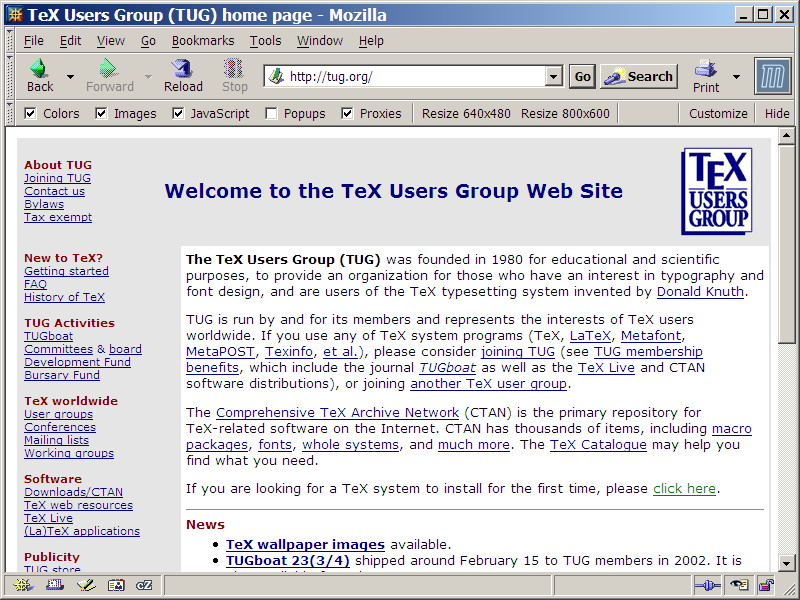
\includegraphics[keepaspectratio,width=\hsize,height=\halfh]
{images/tugorg.png}

\caption[TeX Users Group web site]{
The web site of the TeX Users Group \citep{TUG}.
\imgcredit{Screenshot taken by the author of this thesis.}
}
\label{fig:TUG}
\end{figure}




\subsection{Installing \protect\LaTeXe}

For information about availability, versions, installation, etc. of
\LaTeXe\ consult the online
\emph{TeX Frequently Asked Questions} \citep{TeXfaq}.
%
The best way to install \LaTeXe\ under Windows is to get the TeXLive
2016 \citep{texlive} DVD distribution. You can download an ISO image
from CTAN TeXLive \citep{ctan-texlive}.  Under Windows 10, you can
mount an ISO image by double-clicking, it is no longer necessary to
actually burn the image to a DVD.





\subsection{Installing Extra \protect\LaTeXe Packages}

Depending on the \LaTeXe\ package you install, you may need to install
additional or more recent versions of \LaTeXe\ packages. For example,
this thesis makes use of the \LaTeXe\ \fname{titlesec} package.
%
You can find a list of packages at your local CTAN site \citep{CTAN}.
To install a package, read the advice at
\url{http://www.ctan.org/installationadvice/}





\subsection{Running \protect\LaTeXe}

When running \LaTeXe\ under Unix, check that the environment variables
are set to something like the values shown here:
\begin{samepage}
\begin{lstlisting}
setenv TEXINPUTS .:~/tex/inputs:./inputs::
setenv BSTINPUTS .:~/tex/inputs::
setenv BIBINPUTS .:~/tex/bib:./bib::
\end{lstlisting}
\end{samepage}


\LaTeXe\ updates certain auxiliary files during translation (for
example with figure numbers or captions) and makes use of them in
subsequent runs. To be absolutely certain that all references are
resolved correctly, run \fname{pdflatex}, \fname{biber},
\fname{pdflatex}, and \fname{pdflatex} in sequence, as shown
below for this thesis:
\begin{samepage}
\begin{lstlisting}
pdflatex thesis
biber thesis
pdflatex thesis
pdflatex thesis
\end{lstlisting}
\end{samepage}




An alternative is to use the \fname{latexmk} perl script:
\begin{samepage}
\begin{lstlisting}
latexmk --pdf thesis
\end{lstlisting}
\end{samepage}


\fname{latexmk} can also be configured using a config file such as
\lstinline|$HOME/.latexmkrc| in the user's home directory: % dummy comment $
\begin{samepage}
\begin{lstlisting}[language=Perl,]
$pdf_mode = 1;  # force use of pdflatex
\end{lstlisting}   % dummy comment $
\end{samepage}


% latexmk
% http://www.ctan.org/pkg/latexmk/
% http://users.phys.psu.edu/~collins/software/latexmk-jcc/
% http://users.phys.psu.edu/~collins/software/latexmk-jcc/latexmk-437.pdf




\subsection{Spell Checking}

GNU Aspell \citep{Aspell} is a free open source spell checker.  It can
automatically ignore \LaTeXe\ commands. Aspell can either be run from
the command line or integrated into other packages such as Emacs.





\subsection{Integrated Development Environments (IDEs) for \protect\LaTeXe}

Under Windows you might want to use an integrated development
environment (a fancy editor) for \LaTeXe, which have built-in support
for editing \LaTeXe, spell checking, compiling, and so forth.
The IDEs assume that you have a working \LaTeXe installation,
so install \LaTeXe first.
%
The best are Texmaker \citep{texmaker}, TeXnicCenter
\citep{TeXnicCenter} (shown in Figure~\ref{fig:TeXnicCenter}), and LEd
\citep{LEd}, all of which are free. The shareware WinEdt
\citep{WinEdt} is also very good.


\begin{figure}[tp]
\centering
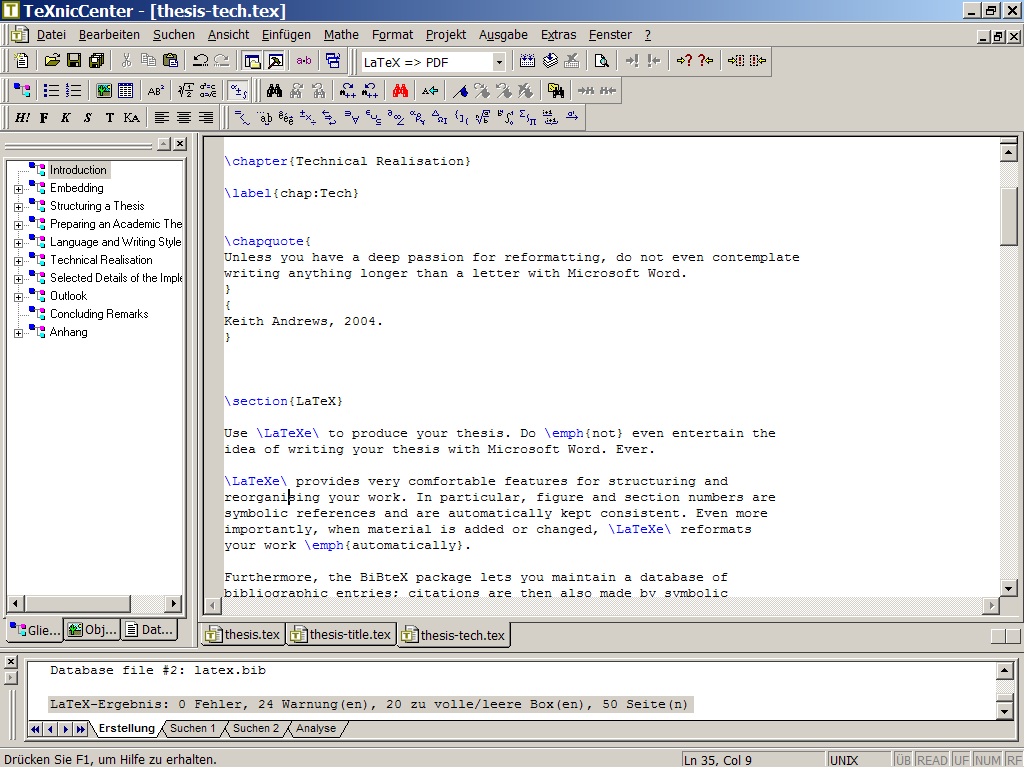
\includegraphics[keepaspectratio,width=\hsize,height=\halfh]
{images/texnic.png}

\caption[The TeXnicCenter IDE]{
The TeXnicCenter \citep{TeXnicCenter} integrated development
environment (IDE) for \LaTeXe.
\imgcredit{Screenshot taken by the author of this thesis.}
}
\label{fig:TeXnicCenter}
\end{figure}








\section{Including Images}

Use the \fname{graphicx} package to include images:
\begin{samepage}
\begin{lstlisting}
\usepackage{graphicx}
\end{lstlisting}
\end{samepage}



\subsection{Screenshots}

Screenshots should be made using software such as IrfanView or Gimp
and \emph{saved as PNG}. PNG is a lossless image format which
preserves every pixel of the original image. Sometimes, novices save
screenshots as JPEG (\fname{.jpg}), which is an inherently lossy image
format. Screenshots saved as JPEG invariably introduce artefacts such
as smudged lines and text, due to the way that JPEG achieves its high
compression rates.




\subsection{Diagrams}

Diagrams and illustrations should be drawn using a \emph{vector}
graphics editor such as Adobe Illustrator or
Inkscape\citep{Inkscape}. Archive (and hand-in) the respective source
files (\fname{.ai} or \fname{.svg}). Convert or export the diagram to
PDF for inclusion into \LaTeXe.

Vector graphics are based on objects such as lines, circles, polygons,
and text strings and as such are freely scalable without loss of
quality. In contrast, \emph{raster} graphics are based on pixels and
do not scale without loss of quality. Saving diagrams in a raster
format such as PNG, GIF, or JPEG means they cannot be resized without
considerable loss of quality.





\subsection{Graphs and Plots}

Tabular data can be plotted as, say, a line chart or bar chart, using
the free packages \fname{gnuplot} \citep{gnuplot} or R \citep{R-Project}.
The plots should be created as SVG (vector graphics), which can then
be touched up, cropped, and converted to PDF using Adobe Illustrator
or Inkscape\citep{Inkscape}.





\section{Including Listings}

Use the \vname{listings} package to include source code listings.
There are three types of listing:
\begin{itemize}
\item \liintro{Inline}: A small snippet of code can be contained
  within the flow of a paragraph using \lstinline!\lstinline!, for
  example \lstinline|\lstinline!var i:integer;!| produces
  \lstinline!var i:integer;!.

\item \liintro{In-Place displayed}: An in-place displayed listing is a
  block of code listed at the place where it occurs. Use in-place
  displayed listings for short blocks of source code upto max $n$
  lines (I use $n=3$). Create an in-place displayed listing with the
  \vname{lstlisting} environment, but without using the \vname{float}
  parameter.

\item \liintro{Floating displayed}: A floating displayed listing is a
  block of code treated like other \LaTeXe floats (such as figures or
  tables). Use floating displayed listings for longer blocks of code.
  \LaTeXe places the Listing at some point later on. Create a floating
  displayed listing with the \vname{lstlisting} environment, but
  specify the \vname{float} and \vname{caption} parameters. A floating
  displayed listing is given a number (Listing 2.1) and is listed in
  the List of Listings.

\end{itemize}

The \vname{listings} package is currently not designed for use with
UTF8 characters. To use UTF8 characters inside listings, you have to
specify the parameter \lstinline!inputencoding=utf8! and 
specify each character inside the \lstinline!literate=! parameter
to the \lstinline!\lstset! command.








\section{Biblatex and Biber}

Biblatex \citep{Biblatex} is a companion system to \LaTeXe, which
allows you to manage sets of references in plain text files (called
\fname{.bib} files) and cite references from within your
\LaTeXe\ documents.  Biber \citep{Biber} is a program which takes
\fname{.bib} files and manages the formatting of citations and of the
bibliography itself. Biblatex and Biber have replaced the now obsolete
BibTex.



\cleardoublepage
%----------------------------------------------------------------
%
%  File    :  survey-examples.tex
%
%  Author  :  Keith Andrews, IICM, TU Graz, Austria
% 
%  Created :  18 May 2012
% 
%  Changed :  18 May 2012
% 
%----------------------------------------------------------------

\chapter{Selected Examples of Doing Things with \LaTeXe\
(and Test of Extremely
Long Chapter Titles to See How They Work Or Not)
}

\label{chap:SelectedExamples}


This chapter contains some examples of typical \LaTeXe\
usage.




\section{First Selected Example}

An example of using a table can be seen in Table~\ref{tabBestPubs}.

\begin{table}[tp]
\centering
\begin{tabular}{|llrp{10cm}|}
\hline
Name & Type & Rating & Description \\
\hline
The Office &
English &
***** &
The best pub in Graz. Hidden in the narrow streets
of the old town. A wonderful hideout for ex-pats.
A pint of Guinness for only \euro 3.90.
\\
\hline
Flann O'Brien &
Irish &
**** &
In the centre of town and easy to find for
marauding tourists.
\\
\hline
O'Carolans &
Irish &
**** &
In the centre of town in a small side street next to Flann's.
Small, cosy Irish pub.
\\
\hline
O'Riginal &
pseudo Irish &
 &
Austrian dive pretending to be an Irish pub.
Definitely not my cup of tea.
\\
\hline
\end{tabular}

\caption[Best Pubs in Graz]
{
The best pubs in Graz.
}
\label{tabBestPubs}
\end{table}





\section{Second Selected Example}

This example shows how to inculde vector graphics in the form of PDF
files. It also shows how to use subfigures within a figure.


\begin{figure}[tp]
\centering
\subfloat[
A object has been composed to represent an
abstract version of the clock tower in Graz.
Here, the object is in its initial state.
]
{
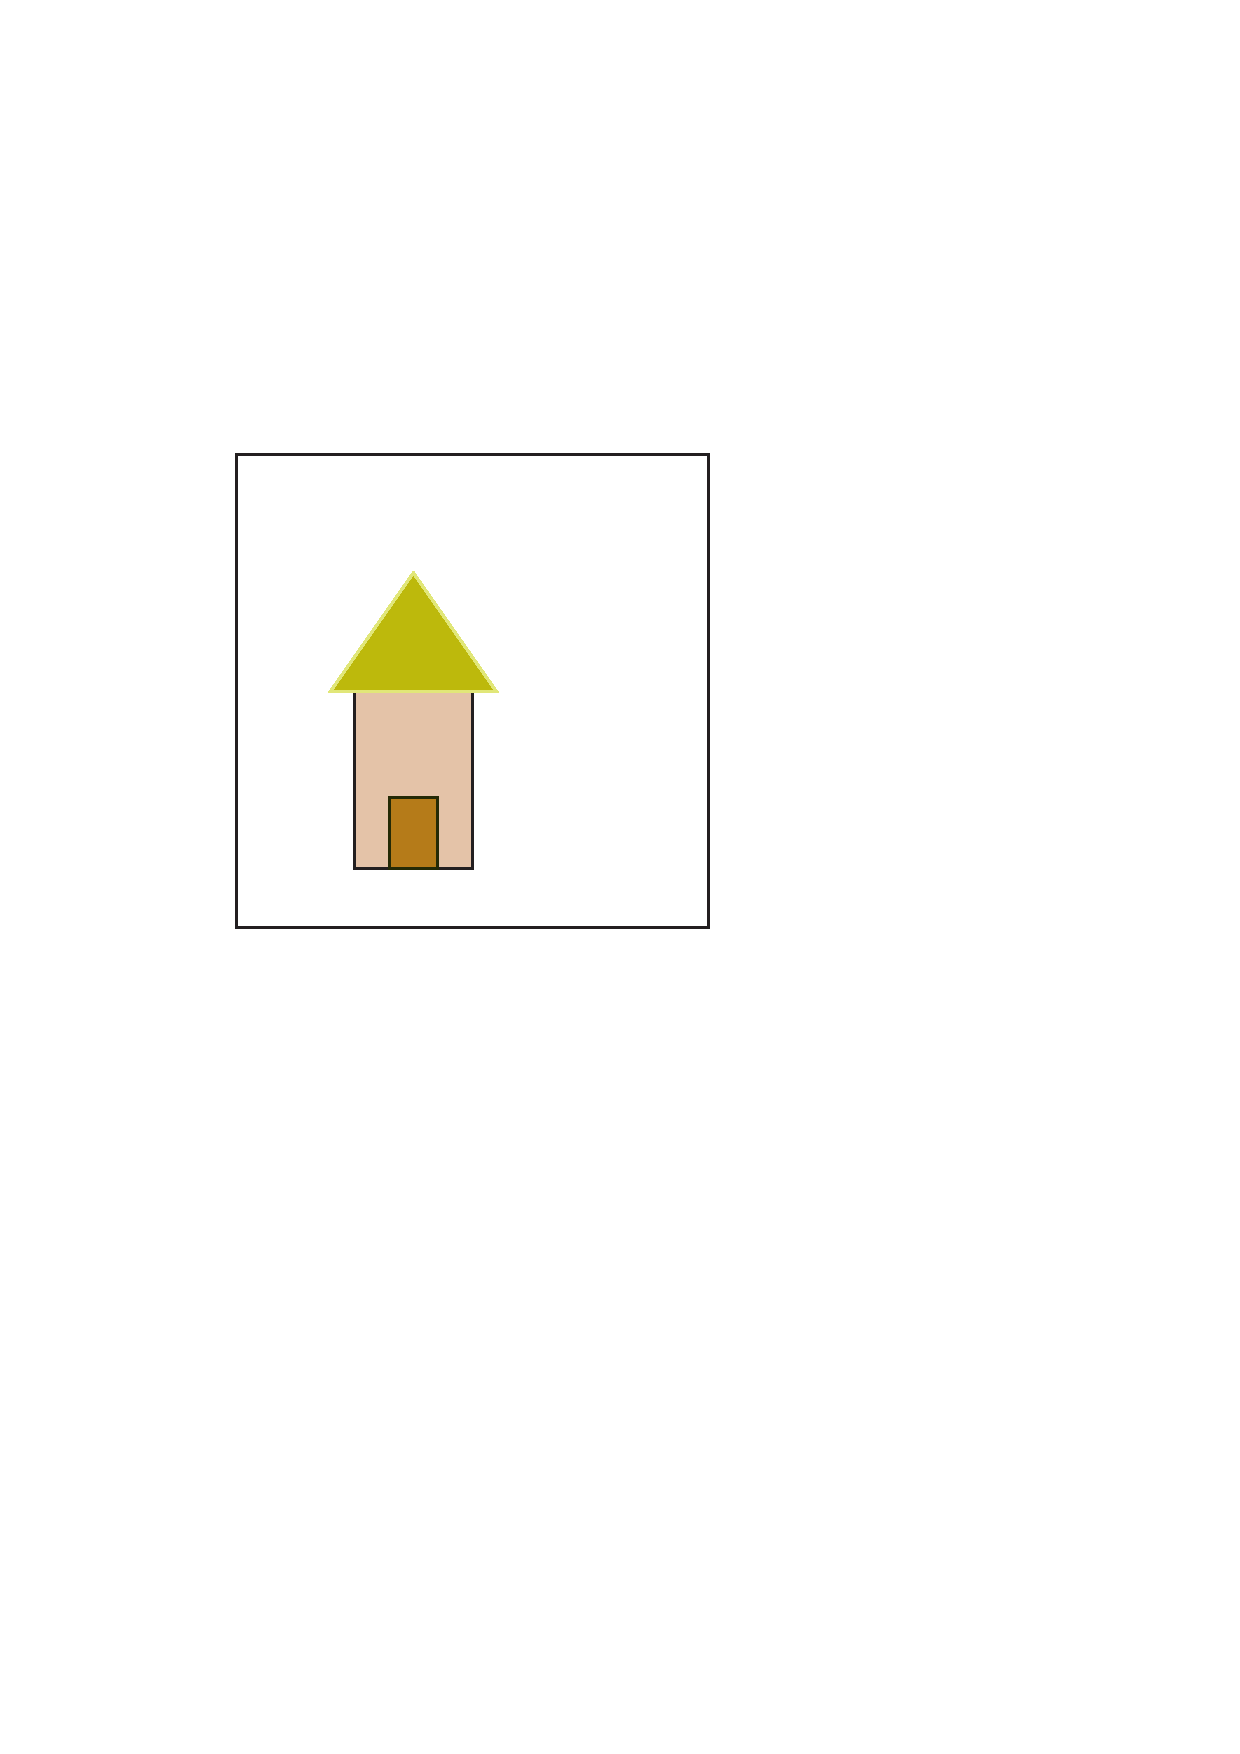
\includegraphics[width=0.45\hsize]{diagrams/multi1}
\label{figTower1}
}
\hfill
\subfloat[
The object has been scaled and rotated, and now resembles
a leaning tower.
]
{
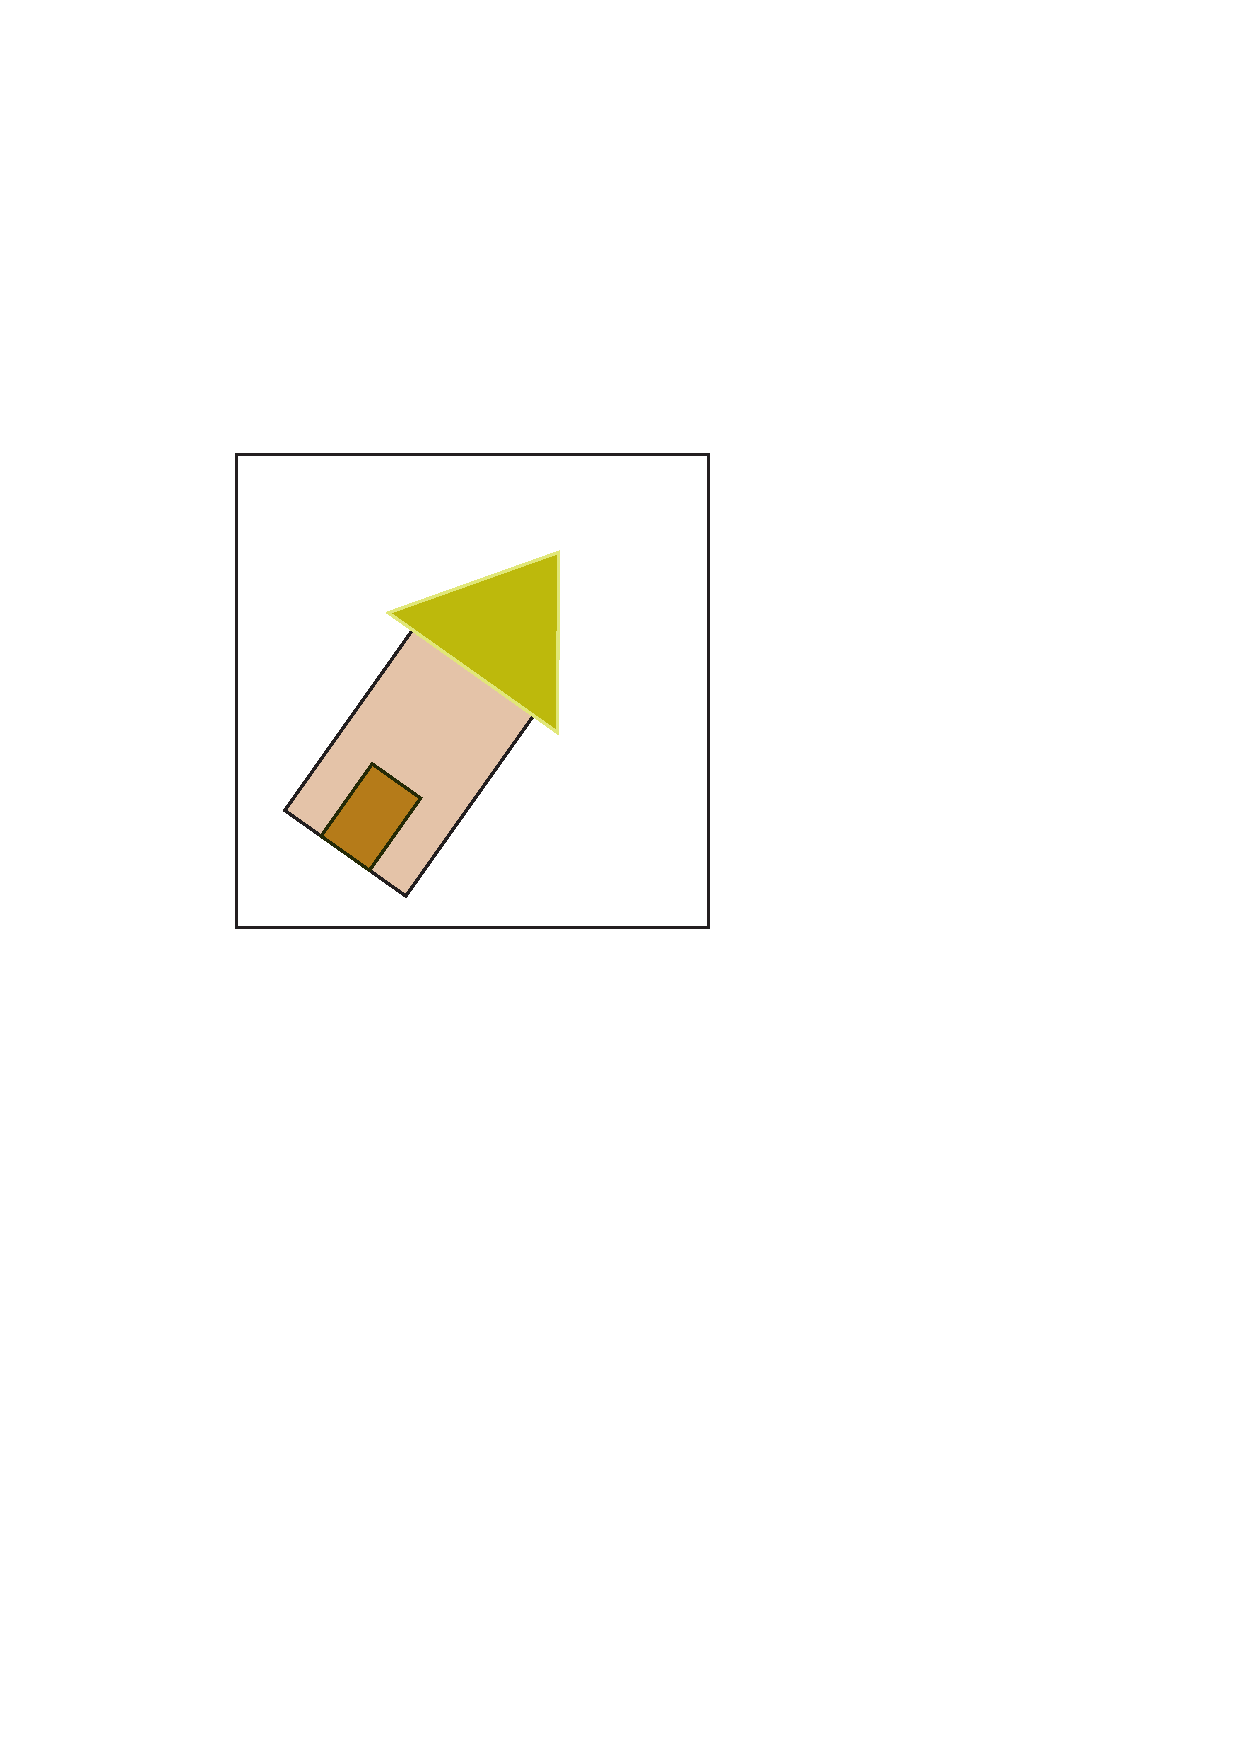
\includegraphics[width=0.45\hsize]{diagrams/multi2}
\label{figTower2}
}

\caption[Abstract Clock Towers]
{
The leaning tower of Graz. An abstract model of the clock
tower in Graz leaning over time. \subref{figTower1} shows
the initial state. \subref{figTower2} shows the final state.
}
\label{figWholeFig}
\end{figure}


An example of using the \vname{subfig} package can be seen in
Figure~\ref{figWholeFig}. Figure~\ref{figTower1} shows the polygons
before transformation, while Figure~\ref{figTower2} shows them
afterwards.




\section{Third Selected Example}


This example shows how to include a screen shot (or other raster
graphic) into a \LaTeXe\ figure.

\begin{figure}[tp]
\centering
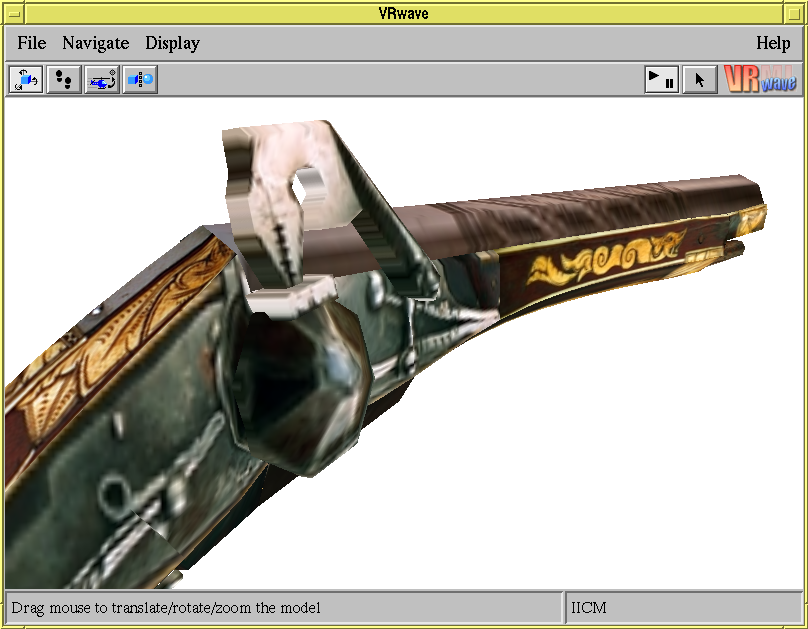
\includegraphics[keepaspectratio,width=\hsize]{images/pist}

\caption[VRwave in Flip Mode]
{%
VRwave in Flip mode displaying a textured model of a cavalry pistol
from the world-renowned Zeughaus (armoury) in Graz.
\imgcredit{Image extracted from \citet[page 81]{Andrews-VRwave}
under the terms of the ACM copyright. \copyrightACM}
}
\label{fig:Pistol}
\end{figure}


An example of how to correctly cite the source when using an image
from someone else. In their 1998 paper, \citet{Andrews-VRwave} discuss
the VRwave VRML browser. Figure~\ref{fig:Pistol} shows a VRML model of
a cavalry pistol from the Armoury in Graz displayed in the VRwave VRML
browser.





\section{Fourth Selected Example}

You can use many (but not all) of the thousands of characters
available in the UTF-8 \citep{Wikipedia-UTF8,Unicode-Charts} character
encoding. For example, the German umlauts (äüö), the German sharp s
(ß), or the yen symbol (¥).

You can also try some of the \approxsym 100 symbols available
in the \vname{textcomp} package, such as the yen symbol (\textyen) and
a circled letter A (\textcircled{A}).

Use the \vname{vname}, \vname{cname}, and \vname{fname} macros to
define the style for variable names, class names, and file names. You
can also define your own macros. The is a very long file name
\fname{/usr/data/keith/travel/austria/vienna.txt} to see how they are
broken at a line end. A typical class name is
\cname{HVSInformationPyramidsInputFactory}.






\section{Fifth Selected Example}

Sometimes, a macro (new command definition) can be useful to define
the contents of table cells, particularly if these contain images. For
example, Table~\ref{tab:WinIconicLang} uses the macro called
\vname{iibox}, which takes a single parameter, the name of
the particular image.



\begin{table}[tp]

\newcommand{\iibox}[1]{\parbox[c][1cm][c]{1cm}{%
\includegraphics[scale=0.6]{./images/icons/#1}
}}

\begin{center}
\begin{tabular}[t]{|p{7cm}c|}
\hline
\multicolumn{2}{|l|}{\sffamily \bfseries Elementary Symbols}            \\
Document                            & \iibox{win-il-gen-doc}            \\
Assistant                           & \iibox{win-il-gen-ass}            \\
Template                            & \iibox{win-il-gen-tmpl}           \\
\hline
\multicolumn{2}{|l|}{\sffamily \bfseries Document Types}                \\
Text document                       & \iibox{win-il-text-doc}           \\
Spreadsheet document                & \iibox{win-il-spreadsheet-doc}    \\
Presentation document               & \iibox{win-il-presentation-doc}   \\
Database document                   & \iibox{win-il-database-doc}       \\
\hline
\multicolumn{2}{|l|}{\sffamily \bfseries Applications}                  \\
Word                                & \iibox{win-il-word-appl}          \\
Excel                               & \iibox{win-il-xls-appl}           \\
Powerpoint                          & \iibox{win-il-ppt-appl}           \\
Access                              & \iibox{win-il-mdb-appl}           \\
\hline
\multicolumn{2}{|l|}{\sffamily \bfseries Generated Icons}               \\
Word text document                  & \iibox{win-il-word-doc}           \\
Excel spreadsheet document          & \iibox{win-il-xls-doc}            \\
Powerpoint presentation document    & \iibox{win-il-ppt-doc}            \\
Access database document            & \iibox{win-il-mdb-doc}            \\[2ex]
%
Word template                       & \iibox{win-il-word-tmpl}          \\
Powerpoint template                 & \iibox{win-il-ppt-tmpl}           \\
Access template                     & \iibox{win-il-mdb-tmpl}           \\[2ex]
%
Word template assistant             & \iibox{win-il-word-ass}           \\
Powerpoint template assistant       & \iibox{win-il-ppt-ass}            \\
Access template assistant           & \iibox{win-il-mdb-ass}            \\[2ex]
%
\hline
\end{tabular}
\end{center}

\caption[Iconic language for Windows NT 4.0 documents]
{
Iconic language for Windows NT 4.0 documents.
}
\label{tab:WinIconicLang}
\end{table}




\section{Textual Citations}

\citet{DataAnalysisChallenges} define visual analytics as:
\begin{quotation}
``iterative process that involves collecting information, data
  preprocessing, knowledge representation, interaction, and decision
  making''.
\end{quotation}


\citet[Chapter~7]{InteractiveDataVisualisation} categorise
visualisation techniques for multi-variate data according to the
graphical primitive used in the rendering: points, lines, and regions.




\cleardoublepage
%----------------------------------------------------------------
%
%  File    :  survey-concl.tex
%
%  Author  :  Keith Andrews, IICM, TU Graz, Austria
% 
%  Created :  27 May 1993
% 
%  Changed :  16 Nov 2010
% 
%----------------------------------------------------------------


\chapter{Concluding Remarks}

\label{chap:Concl}





\cleardoublepage
\printbibliography[heading=bibintoc]




\end{document}

